% ============================================================
%  MERGE — Final Report (ACL Format)
%  Introduction to NLP (S26) — Spring 2026
%  Team: Abhay Sharma, Ankit Kumar, Hritik Ranjan, Vikash Kumar
% ============================================================
\documentclass[11pt]{article}

\usepackage{acl}
\usepackage{times}
\usepackage{latexsym}
\usepackage[T1]{fontenc}
\usepackage[utf8]{inputenc}
\usepackage{microtype}
\usepackage{graphicx}
\usepackage{url}
\usepackage{amsmath}
\usepackage{amssymb}
\usepackage{float}
\usepackage{booktabs}
\usepackage{multirow}
% NOTE: hyperref is already loaded by acl.sty (with breaklinks option).
%       Do NOT add \usepackage{hyperref} here -- it causes option clash.
%       To change link colours, set them AFTER \usepackage{acl}:
\hypersetup{colorlinks=true,linkcolor=blue,urlcolor=blue,citecolor=blue}

\DeclareMathOperator*{\argmax}{arg\,max}

% ----------------------------------------------------------------
\title{MERGE: Multimodal Emotion-Driven Rhythmic Lyric Generation Engine}

% ACL \author{}: use \And for horizontal split between authors.
% \thanks{} is safe for footnotes (GitHub link etc.).
% Do NOT use \url{} or \small directly inside \author{}.
\author{Abhay Sharma \And Ankit Kumar \And Hritik Ranjan \And Vikash Kumar}
  
\begin{document}
\maketitle


\begin{abstract}
Creative language generation has gained increasing attention in natural language 
processing, particularly for tasks such as poetry and song lyric generation. 
However, most existing systems focus either on structural constraints such as 
rhyme and meter or on semantic control mechanisms such as sentiment, topic, 
or style. The integration of multimodal emotional signals with rhythm-aware 
lyric generation remains relatively underexplored.

In this work, we propose \textbf{MERGE} (Multimodal Emotion-Driven Rhythmic 
Lyric Generation Engine), a framework for generating rhythm-aware song lyrics 
conditioned on emotional states inferred from facial expressions. The system 
first detects the user’s emotional state using a facial emotion recognition 
model and then conditions a transformer-based language model on the predicted 
emotion to guide lyric generation. To maintain lyrical structure, rhythm-aware 
constrained decoding is applied to enforce syllable counts and rhyme patterns 
during generation.

We further introduce \textbf{REDS}, a composite evaluation metric designed 
for lyric generation that measures rhythmic consistency, emotional alignment, 
lexical diversity, and semantic coherence. MERGE provides a framework for 
exploring emotion-conditioned lyric generation while preserving structural 
properties of song lyrics.\end{abstract}




\section{Introduction}

The motivation of this project is to develop an emotion-aware system 
capable of generating creative musical content based on a user's 
emotional state inferred from sensory inputs. Direct music synthesis 
conditioned on physiological or multimodal sensor data poses significant 
challenges due to limited dataset availability, the high dimensionality 
of audio generation, and the complex alignment between emotional intent 
and musical structure \cite{cao2022multi}. To preserve the objective of 
emotion-driven creative generation while remaining within the methodological 
scope of natural language processing (NLP), this work reformulates the 
problem as emotion-conditioned lyric generation.

Facial emotion recognition provides a practical and widely studied 
modality for sensing emotional states \cite{goodfellow2013challenges, li2017reliable}.
 At the same time, song lyrics serve as a primary textual medium through which 
 emotional expression is conveyed in music. These properties make lyrics a 
 suitable domain for studying emotion-controlled and structurally constrained 
 language generation. Prior research in NLP has explored emotion-conditioned 
 text generation as well as structural constraints such as rhyme schemes and 
 syllable patterns in poetry and lyric generation. However, these directions 
 have largely been investigated independently.

A key challenge in emotion-conditioned lyric generation lies in the 
limited availability of large-scale lyric datasets with explicit 
emotion annotations. While curated datasets such as the Spotify 
Million Playlist Dataset \cite{devdope_2023_spotify_900k} provide 
approximately 500k lyrics annotated with emotional labels, their scale 
remains limited for training modern neural language models. To 
address this limitation, this work leverages large-scale lyric corpora 
obtained from the Genius lyric dataset \cite{lim2021expertise}, which 
provides substantially larger collections of song lyrics. Since explicit 
emotion annotations are not available for these datasets, we construct 
emotion labels using a scalable annotation pipeline that aggregates 
predictions from a GoEmotions-based classifier and maps fine-grained 
emotional categories into the six facial emotion recognition (FER) classes 
through normalization and weighted line-level aggregation. This procedure 
enables the creation of large-scale emotion-labeled lyric datasets suitable 
for training emotion-conditioned language models.

While prior work has examined controlled text generation and rhythm-aware 
lyric generation separately, the integration of facial emotion signals as 
control inputs for rhythm-aware lyric generation remains relatively 
underexplored, particularly in English-language songwriting. Bridging 
this gap requires a framework that can incorporate visual emotional 
cues into the generation process while maintaining the structural 
characteristics that define song lyrics.

In this work, we propose 
\textbf{MERGE (Multimodal Emotion-Driven Rhythmic Lyric Generation Engine)}, 
a multimodal framework that connects facial emotion recognition with 
rhythm-aware lyric generation. MERGE uses facial emotion recognition 
models to infer emotional states from visual inputs and employs these 
signals to condition a transformer-based language model trained on 
large-scale lyric corpora. To ensure structural coherence, 
the generation process incorporates rhythm-aware decoding constraints
 based on syllable counts and rhyme schemes.

This work investigates two central research questions: (1) whether facial emotion signals can effectively serve as control inputs for lyric generation, and (2) whether rhythmic constraints such as syllable count and rhyme can be enforced during decoding in emotion-conditioned lyric generation without degrading emotional alignment or linguistic fluency.
The contributions of this work are fourfold: 
(1) MERGE, a multimodal framework that connects facial emotion recognition
 with lyric generation, 
(2) a scalable lyric emotion annotation pipeline that maps fine-grained 
GoEmotions predictions to facial emotion recognition (FER) categories using 
normalization and weighted aggregation, enabling large-scale emotion labeling
 of lyric corpora, 
(3) a rhythm-aware constrained decoding strategy for maintaining lyrical
 structure during generation, and 
(4) REDS, a composite evaluation metric designed for assessing emotional 
alignment and structural quality in generated lyrics.

The source code and implementation details for this project are available
 at the following link.\footnote{\url{https://github.com/IIITH-2025-27/NLP_Project}}


\section{Related Work}

\textbf{Facial Emotion Recognition.}
Facial emotion recognition has achieved strong performance using deep 
convolutional neural networks, with architectures such as ResNet 
and MobileNet commonly evaluated on benchmark datasets including 
FER-2013 and RAF-DB \cite{goodfellow2013challenges, li2017reliable}. 
The FER-2013 dataset, introduced as part of a large-scale representation 
learning challenge, contains over 35,000 grayscale facial images annotated 
with basic emotion labels such as angry, disgust, fear, happy, sad, surprise,
and neutral \cite{goodfellow2013challenges}. Due to its accessibility and 
scale, FER-2013 remains one of the most widely used benchmarks for training 
and evaluating facial emotion recognition systems. More recent research has 
explored transformer-based architectures and multimodal fusion networks for 
emotion recognition, improving the ability of models to capture contextual 
emotional signals from visual data \cite{zhang2023multimodal}. These advances
make facial emotion recognition sufficiently reliable to serve as an emotion 
sensing component in downstream generative systems.

\textbf{Controlled Text Generation.}
In natural language processing, controlled text generation has been widely 
studied as a mechanism for steering language models toward desired attributes 
such as sentiment, topic, or style. Early approaches relied on conditional
fine-tuning strategies and control tokens for large language models 
\cite{radford2019language}. More recent work has explored attribute-guided
generation techniques that allow large language models to produce text aligned 
with specific semantic properties, including emotional tone and stylistic 
constraints \cite{hu2023attribute}. These approaches demonstrate that 
external control signals can effectively influence the behavior of 
generative language models.

\textbf{Lyric and Poetry Generation.}
Research on poetry and lyric generation has extensively explored methods
for enforcing structural constraints such as rhyme schemes, meter, and 
syllable counts. Early approaches relied on rule-based techniques and 
phonetic resources such as the CMU Pronouncing Dictionary to analyze
syllable patterns and rhyming structures 
\cite{ghazvininejad2016generating, gonccalo2024automatic}. More recent
neural approaches incorporate such constraints during generation to 
produce structurally coherent poetic text. However, most existing 
systems primarily focus on structural control and do not explicitly i
nvestigate how these rhythmic constraints interact with emotion-conditioned
generation, particularly when emotional signals originate from external
modalities such as facial expressions. Neural approaches later introduced 
sequence-to-sequence and transformer-based architectures capable 
of generating structured poetic text. More recent lyric generation
systems incorporate musical or prosodic signals to guide the generation process. 
For example, SongRewriter \cite{sun2023songrewriter} employs a randomized
multi-level masking strategy to enable both lyric generation and editing
while incorporating keyword prompts and vowel modeling tasks to encourage
flexible rhyme schemes. XAI-Lyricist \cite{liang2024xai} conditions lyric
generation on musical prosody signals to improve singability while also 
providing interpretable explanations for rhythmic alignment.

\textbf{Collaborative and Multimodal Generation Systems.}
Another emerging direction explores collaborative or multi-agent 
architectures for lyric generation. Liu et al. \cite{liu2024agent} 
propose a multi-agent system in which different agents handle specialized 
tasks such as rhyme suggestion, syllable control, and lyric–melody 
alignment. Similarly, Ram et al. \cite{ram2021say} employ multitask
transfer learning with the T5 transformer model to model lyrical 
constraints including beat alignment and target word endings.
More broadly, recent multimodal generative models such as MusicLM 
\cite{huang2023musiclm} demonstrate the potential of combining 
semantic signals with generative models for music-related tasks, 
although these systems primarily focus on audio generation rather
than lyric generation.

Despite these advances, most existing systems either focus on 
structural lyric generation or rely on musical signals such 
as melody or prosody as conditioning inputs. The integration 
of visual emotion signals—such as facial expressions—with 
rhythm-aware lyric generation remains relatively underexplored,
particularly in English-language songwriting. MERGE addresses
this gap by providing an end-to-end framework that connects facial 
emotion recognition with constrained lyric generation.



% ============================================================
\section{Dataset Details}
% ============================================================

\subsection{Lyric Corpus}

Lyrics are sourced from the \textbf{Genius} corpus
\cite{lim2021expertise}, which contains songs spanning
many languages.  After filtering for English-language content,
approximately \textbf{3.2 million} songs remain.  A cleaned
version of this corpus is publicly available on
Kaggle.\footnote{\url{https://www.kaggle.com/datasets/ankit477/genius-dataset-cleaned}}



\subsection{Facial Expression Datasets}

The FER component is trained on a unified corpus comprising
three publicly available datasets:

\begin{itemize}
  \item \textbf{FER-2013} \cite{goodfellow2013challenges}:
        35{,}887 grayscale 48$\times$48 images, seven original
        classes (disgust excluded, yielding six classes).
  \item \textbf{RAF-DB} \cite{li2017reliable}: $\sim$15{,}339
        real-world images with basic and compound emotion labels
        (disgust excluded), It was found on kaggle.\footnote{\url{https://www.kaggle.com/datasets/shuvoalok/raf-db-dataset}}
  
        \item \textbf{AffectNet} \cite{mollahosseini2019affectnet}:
        $\sim$450{,}000 images annotated with eight emotions. But out of them 
        only $\sim$30{,}000 was used for training (disgust excluded), which were found on kaggle.\footnote{\url{https://www.kaggle.com/datasets/mstjebashazida/affectnet}}
\end{itemize}

A unified six-class mapping
$\mathcal{E}=\{\textit{angry},\textit{fear},\textit{happy},
\textit{sad},\textit{surprise},\textit{neutral}\}$
is defined across all three sources.  The disgust and contempt
categories are excluded because they appear rarely in song
lyrics and their linguistic expression substantially overlaps
with anger and sadness. Additionally, FER-2013 and other datasets contain very
few disgust, contempt, and surprise samples, resulting in a severe class imbalance.

\subsection{Dataset Construction and Emotion Mapping}
\label{sec:dataset}

Large-scale lyric datasets typically lack explicit emotion 
annotations, which makes it difficult to train emotion-conditioned 
language models. To address this limitation, we construct an 
emotion-labeled lyric dataset using an automatic annotation pipeline 
as shown in Figure \ref{fig:dataset_pipeline}.




Lyrics are collected from large public lyric corpora, specifically the Genius dataset \cite{lim2021expertise}, which contains lyrics in many languages out of which approx 3.2 million belongs to English language. Emotional signals are inferred using a pretrained emotion classifier based on the RoBERTa architecture\cite{lowe2023roberta}, which is fine-tuned on the GoEmotions dataset \cite{demszky2020goemotions}. The GoEmotions label space contains $28$ categories, consisting of $27$ fine-grained emotion labels and one neutral category. For each input lyric line, the classifier outputs a probability distribution over these $28$ labels, which serves as the basis for constructing the emotion representations used in the subsequent stages of the pipeline.

To ensure compatibility between textual emotions and facial emotion recognition outputs, the fine-grained emotion space is mapped into a smaller set of basic emotions, inspired by the circumplex model of affect and theories of basic emotions \cite{russell1980circumplex, ekman1992argument}. The emotion space is reduced to the following set
\[
\mathcal{E} =
\{\text{angry}, \text{fear}, \text{happy}, \text{sad}, \text{surprise}, \text{neutral}\}.
\]

\vspace{-0.7cm}
\begin{figure}[H]
\centering

\includegraphics[width=0.9\linewidth]{diagram2.pdf}
\caption{Pipeline for constructing the emotion-labeled lyric dataset.}
\label{fig:dataset_pipeline}
\end{figure}
\vspace{-0.3cm}

The disgust category is excluded for two reasons. First, explicit expressions of disgust rarely occur in song lyrics and are often linguistically expressed as sadness or disappointment. Second, the FER-2013 facial emotion dataset contains very few samples labeled as disgust, resulting in severe class imbalance during model training. To maintain a consistent emotion space across modalities, disgust-related signals are therefore merged into the sadness category.
The created dataset is being hosted on kaggle\cite{author2025}.



\subsection{Lyric Dataset and Emotion Labeling}
Each song is segmented into individual lyric lines. Let a song contain $n$ lyric lines, where the index of a line is denoted by
\[
i \in \{1,2,\dots,n\}.
\]


For each lyric line $i$, the GoEmotions classifier produces a probability vector over the $28$ emotion labels:
\[
\mathbf{p}_i =
\left[
p_i^{(1)}, p_i^{(2)}, \dots, p_i^{(28)}
\right] \in \mathbb{R}^{28},
\]
where $p_i^{(e)}$ denotes the probability assigned to label $e$ and satisfies
\[
0 \le p_i^{(e)} \le 1.
\]

To obtain emotion representations compatible with facial emotion recognition categories, the fine-grained emotion labels are grouped into six emotion sets:
\[
\begin{aligned}
A &= \{\text{anger}, \text{annoyance}, \text{disapproval}\}, \\
F &= \{\text{fear}, \text{nervousness}\}, \\
H &= \{\text{admiration}, \text{amusement}, \text{approval}, \text{caring}, \\
  &\quad \text{desire}, \text{excitement}, \text{gratitude}, \text{joy}, \text{optimism}, \\
  &\quad \text{love}, \text{pride}, \text{relief}\}, \\
S &= \{\text{sadness}, \text{grief}, \text{disappointment}, \text{remorse}, \\
  &\quad \text{disgust}\}, \\
U &= \{\text{surprise}, \text{realization}\}, \\
N &= \{\text{neutral}, \text{curiosity}, \text{confusion}\}.
\end{aligned}
\]

Using these groups, the emotion score for each category is computed by summing probabilities belonging to the same group. For example, the anger score for line $i$ is defined as
\[
q_i^{\text{angry}} =
\sum_{e \in A} p_i^{(e)}.
\]

Applying the same procedure to all emotion groups produces a six-dimensional emotion vector for lyric line $i$:
\[
\mathbf{q}_i =
\left[
q_i^{\text{angry}},
q_i^{\text{fear}},
q_i^{\text{happy}},
q_i^{\text{sad}},
q_i^{\text{surprise}},
q_i^{\text{neutral}}
\right].
\]

Because multiple probabilities are aggregated, the resulting vector is normalized to obtain a valid probability distribution:
\[
\mathbf{q}_i =
\frac{\mathbf{q}_i}
{\sum_{k=1}^{6} q_i^{(k)}}.
\]

Lyrics often contain narrative lines with little emotional content. To reduce their influence, each line is assigned an emotional weight defined as
\[
w_i = 1 - q_i^{\text{neutral}},
\]
where $w_i$ represents the emotional intensity of lyric line $i$.

The final emotion representation of a song is computed by aggregating the line-level emotion vectors using weighted averaging:
\[
\mathbf{E}_{\text{song}}
=
\frac{\sum_{i=1}^{n} w_i \mathbf{q}_i}
{\sum_{i=1}^{n} w_i}.
\]

The dominant emotion of the song is defined as
\[
e^* =
\arg\max_k
\mathbf{E}_{\text{song}}^{(k)},
\]
where $\mathbf{E}_{\text{song}}^{(k)}$ denotes the score of emotion category $k$.

% ============================================================
\section{Methodology}
% ============================================================

This work proposes an end-to-end multimodal framework that connects 
facial emotion recognition with emotion-conditioned and 
rhythm-aware lyric generation. The system
(as shown in Figure \ref{fig:merge_pipeline}) first detects 
emotional states from facial inputs and then uses these signals to 
guide lyric generation while enforcing linguistic and rhythmic 
constraints such as rhyme patterns and syllable structure.


\begin{figure}[H]
  \centering
  
\includegraphics[width=0.95\linewidth]{diagram1.pdf}
  \caption{Overview of the MERGE framework.  A face image is
           processed by the FER ensemble to produce an emotion
           control token, which is prepended to the lyric
           sequence for GPT-2 fine-tuning.  Rhythm-constrained
           decoding enforces syllable counts and rhyme schemes
           at inference.}
  \label{fig:merge_pipeline}
\end{figure}

\vspace{-0.3cm}

\subsection{Facial Emotion Conditioning}

The MERGE framework uses facial expressions as the emotional input signal for lyric generation. Given a facial image, a facial emotion recognition model predicts the emotional state of the user (as shown in Figure \ref{fig:vision_pipeline}), which is then used to condition the lyric generation process.

The facial emotion recognition model is trained on the FER-2013 
dataset \cite{goodfellow2013challenges}, which contains 35,887 
grayscale facial images labeled with basic emotion categories.
Due to the severe class imbalance of the disgust category in FER-2013, 
the task is reformulated as a 6-class classification problem. The final 
emotion set used in this work is angry, fear, happy, sad, surprise, neutral.


Let $I$ denote the input facial image and let $f_{\theta}$ represent the facial emotion recognition model parameterized by $\theta$. The model produces a vector of logits

\[
\mathbf{z} = f_{\theta}(I)
\]

where $\mathbf{z} \in \mathbb{R}^{6}$ represents the unnormalized scores corresponding to the six emotion categories.

The probability distribution over emotions is computed using the softmax function

\[
P(e_k \mid I) =
\frac{\exp(z_k)}
{\sum_{j=1}^{6} \exp(z_j)}
\]

where $e_k \in \mathcal{E}$ denotes the $k$-th emotion category and $z_k$ represents the corresponding logit value.

The predicted facial emotion is obtained by selecting the class with the highest probability

\[
e^{*} =
\arg\max_{e_k \in \mathcal{E}}
P(e_k \mid I)
\]

The predicted emotion $e^{*}$ is then used as the conditioning signal for the lyric generation model. During inference, this emotion is converted into a control token (for example \texttt{\textless sad\textgreater}) which is prepended to the input sequence of the language model. This allows the model to generate lyrics that are aligned with the emotional state inferred from the user's facial expression.

\begin{figure}[H]
\centering
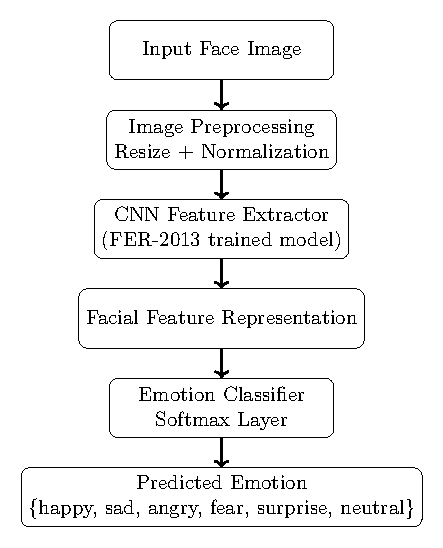
\includegraphics[width=0.9\linewidth]{diagram3.pdf}
\caption{Pipeline of the facial emotion recognition module.}
\label{fig:vision_pipeline}
\end{figure}
\vspace{0.25cm}

\subsection{Emotion-Conditioned Language Model}

Lyric generation is formulated as a controlled text generation task in which emotional context influences the semantic content of generated lyrics. We fine-tune the GPT-2 language model \cite{radford2019language} on the emotion-labeled lyric dataset constructed in the previous subsection.

Emotion conditioning is implemented using explicit control tokens representing the target emotion category. During training, an emotion token (for example \texttt{\textless EMO\_sad\textgreater}) is prepended to each lyric sequence so that the model can learn associations between emotional states and linguistic patterns.

Let
\[
x = (x_1, x_2, \dots, x_T)
\]
denote a lyric token sequence of length $T$, and let $e$ represent the conditioning emotion label. The model learns the conditional probability
\[
P(x \mid e)
=
\prod_{t=1}^{T}
P(x_t \mid x_{<t}, e),
\]
where $x_t$ denotes the token generated at step $t$ and $x_{<t}$ represents the previously generated tokens.

The model is trained using the standard cross-entropy objective for next-token prediction.

\subsection{Rhythm-Constrained Decoding}

To enforce rhythmic and rhyming structure during lyric generation, constrained decoding is applied. The CMU Pronouncing Dictionary provides phonetic representations that allow syllable counting and rhyme detection \cite{cmudict}.

Each generated lyric line must satisfy predefined structural constraints such as a target syllable count and a specified rhyme scheme (for example AABB or ABAB). During decoding, candidate tokens that violate these constraints are filtered from the vocabulary.

When a rhyming token is required at the end of a line, the candidate token set is restricted to words whose phonetic representations match the desired rhyme pattern. Hard constraints enforce structural consistency within each line, while soft back-off strategies allow constraint relaxation or line regeneration if decoding becomes infeasible.

By integrating these constraints directly into the decoding process rather than applying them as post-processing steps, the system generates lyrics that maintain both rhythmic structure and semantic coherence.



% ============================================================
\section{Evaluation Metric: REDS}
% ============================================================


Evaluating creative language generation is challenging because traditional metrics such as BLEU or ROUGE primarily measure lexical overlap and often fail to capture important qualities of lyrics such as emotional alignment, rhythmic structure, and semantic coherence. To address this limitation, we introduce a composite evaluation metric called \textbf{REDS}, designed specifically for emotion-conditioned lyric generation.

REDS evaluates generated lyrics across four complementary dimensions: rhythmic consistency, emotional alignment, lexical diversity, and semantic coherence.

\subsection{REDS Evaluation Metric}

Let a generated lyric consist of $n$ lines

\[
L = {l_1, l_2, \dots, l_n}.
\]

The REDS score is computed as a weighted combination of four components:

\[
\text{REDS} =
\alpha R + \beta E + \gamma D + \delta S
\]

subject to the normalization constraint

\[
\alpha + \beta + \gamma + \delta = 1.
\]

Here $R$, $E$, $D$, and $S$ denote rhythm consistency, emotional alignment, lexical diversity, and semantic coherence respectively, while $\alpha$, $\beta$, $\gamma$, and $\delta$ represent weighting coefficients.

\subsubsection{Rhythm and Rhyme Consistency ($R$)}

Rhythmic structure is evaluated using syllable counts and rhyme patterns derived from phonetic representations in the CMU Pronouncing Dictionary \cite{cmudict}. Let $s_i$ denote the number of syllables in lyric line $l_i$, and let $s^*$ denote the target syllable count for the desired rhythmic pattern.

The syllable consistency score is defined as

\[
R_{\text{syllable}} =
1 -
\frac{1}{n}
\sum_{i=1}^{n}
\frac{|s_i - s^*|}{s^*}.
\]

Rhyme consistency is evaluated by checking whether each line satisfies the expected rhyme scheme. Let

\[
r_i =
\begin{cases}
    1 & \text{if line } l_i \text{ satisfies the rhyme scheme}, \\
    0 & \text{otherwise}.
\end{cases}
\]

The final rhythm score combines both syllable and rhyme correctness:

\[
R =
\frac{1}{2}
\left(
R_{\text{syllable}}
+
\frac{1}{n}
\sum_{i=1}^{n} r_i
\right).
\]

\subsubsection{Emotional Alignment ($E$)}

Emotional alignment measures how well the generated lyrics reflect the intended conditioning emotion. An independent emotion classifier trained on the GoEmotions dataset \cite{demszky2020goemotions} is used to estimate the emotion distribution of the generated text.

Let

\[
\mathbf{p} =
[p_1, p_2, \dots, p_K]
\]

denote the predicted probability distribution over the emotion set

\[
\mathcal{E} =
{\text{angry}, \text{fear}, \text{happy}, \text{sad}, \text{surprise}, \text{neutral}}.
\]

If the intended emotion is $e^*$, the emotional alignment score is defined as

\[
E = p_{e^*}.
\]

\subsubsection{Lexical Distinctiveness ($D$)}

Lexical diversity is measured using distinct n-gram statistics. Let $U_k$ denote the number of unique $k$-grams in the generated lyrics and let $T_k$ denote the total number of $k$-grams.

The distinct-$k$ score is defined as

\[
\text{Distinct}_k =
\frac{U_k}{T_k}.
\]

The lexical diversity score is computed as

\[
D =
\frac{\text{Distinct}_1 + \text{Distinct}_2}{2}.
\]

\subsubsection{Semantic Coherence ($S$)}

Semantic coherence measures the topical consistency between consecutive lyric lines. Let $\mathbf{v}_i$ denote the sentence embedding of line $l_i$ obtained using a pretrained sentence embedding model.

The semantic coherence score is defined as the average cosine similarity between consecutive lines:

\[
S =
\frac{1}{n-1}
\sum_{i=1}^{n-1}
\frac{\mathbf{v}*i \cdot \mathbf{v}*{i+1}}
{|\mathbf{v}*i| |\mathbf{v}*{i+1}|}.
\]

\subsubsection{Normalization}

Each component score is normalized to the interval

\[
R, E, D, S \in [0,1].
\]

This ensures that the evaluation components operate on comparable scales and prevents any single component from dominating the overall metric.

Consequently, the REDS metric is bounded by

\[
0 \le \text{REDS} \le 1.
\]

\subsubsection{Weight Optimization}

The weighting coefficients $\alpha$, $\beta$, $\gamma$, and $\delta$ determine the relative importance of each evaluation component. Rather than selecting these weights manually, they are estimated using correlation-based optimization with human evaluation scores.

Let $H$ denote the vector of human evaluation ratings for generated lyrics. The optimal weights are obtained by maximizing the correlation between REDS scores and human judgments:

\[
(\alpha,\beta,\gamma,\delta) = 
\arg\max
\rho(\text{REDS}, H),
\]

where $\rho(\cdot)$ denotes Spearman's rank correlation coefficient.

This optimization ensures that the REDS metric aligns with human judgments of lyric quality.
Since this work is currently in progress, the REDS metric is proposed as the evaluation framework for lyric generation. The final weighting parameters $\alpha$, $\beta$, $\gamma$, and $\delta$ will be estimated using correlation with human evaluation scores during the final stage of the project.


% ============================================================
\section{Experiments and Training Setup}
% ============================================================

\subsection{Facial Emotion Recognition}

\paragraph{Phase I--IV (ResNet Baseline).}
Phases~I--IV were conducted on Kaggle with GPU acceleration. Phase~I trained ResNet18 via a 243-combination grid search, establishing Adam with $\text{lr}=5\times10^{-5}$ and medium augmentation as baseline ($\approx$62\% test accuracy). Phase~II upgraded to ResNet34 (62.6\%) over 20 epochs with linear warmup (2 epochs), exposing persistent overfitting (8.5\% gap). Phase~III introduced ResNet50 with progressive unfreezing (head trained first, then full model), label smoothing ($\varepsilon=0.1$), dropout, and Cosine Annealing over 25 epochs (3 warmup), reducing the gap to 4.5\% and raising accuracy to 66.8\%. Phase~IV reformulated as six-class classification (removing severely imbalanced \textit{disgust} class) trained for 25 epochs with identical settings, yielding the best single-model result of \textbf{67.43\%} (weighted F1 $=$ 0.671).

\paragraph{Phase V (Multi-Dataset Ensemble).}
To improve generalization beyond FER-2013, Phase~V unifies FER-2013 (35{,}887 images),
RAF-DB ($\sim$15{,}000 images), and AffectNet ($\sim$30{,}000 images) 
into a six-class label space with 80/10/10 split before augmentation 
and MTCNN face filtering \cite{zhang2016joint}. The training set is expanded
using domain-bridging augmentations (RandomGrayscale $p=0.3$, 
GaussianBlur, ColorJitter, RandomAffine, RandomPerspective) for better generalization. 
EfficientNet-B3 and DenseNet-121 is trained individually on Kaggle GPU resources with progressive 
unfreezing over 30 epochs (5 warmup, Cosine Annealing scheduler, head first then 
backbone lr $=10^{-4}$, head lr $=10^{-3}$), Focal Loss \cite{lin2017focal} 
($\gamma=2$) with label smoothing ($\varepsilon=0.1$).
Final predictions: test-time augmentation generates prediction 
sets per model, then ensemble averaging combines them via weighted 
averaging:  $0.6\cdot\hat{p}_{\text{EfficientNet}} + 0.4\cdot\hat{p}_{\text{DenseNet}}$.


\subsection{Language Model Fine-Tuning}

GPT-2 was fine-tuned on the emotion-labeled lyric dataset
using emotion control tokens prepended to each sequence.
Training was conducted on a subset of the annotated corpus
using the AdamW optimizer, a linear warmup schedule, and a
sequence length of 512 tokens.  Six separate models were
trained---one per emotion class---to provide fine-grained
control.

% \begin{table}[h]
% \centering\small
% \begin{tabular}{lp{0.68\columnwidth}}
% \toprule
% \textbf{Emotion} & \textbf{Sample Generated Lyric (excerpt)} \\
% \midrule
% Happy   & \textit{``The sun is bright, the world is free, I
%           feel the joy inside of me''} \\
% Sad     & \textit{``The night is cold, the tears fall down, I
%           hear the silence of the town''} \\
% Angry   & \textit{``I break the chains, I feel the rage, I
%           burn the words upon the page''} \\
% Fear    & \textit{``The dark surrounds, I cannot see, I'm lost
%           within this misery''} \\
% Surprise& \textit{``The world has changed, I can't believe, a
%           new beginning I receive''} \\
% Neutral & \textit{``The road goes on through hill and plain,
%           the seasons turn and come again''} \\
% \bottomrule
% \end{tabular}
% \caption{Sample GPT-2 outputs per emotion condition.
%          Outputs reflect distinct lexical and thematic
%          differences across emotion categories.}
% \label{tab:samples}
% \end{table}


% ============================================================
\section{Results}
% ============================================================

\subsection{Facial Emotion Recognition}

Table~\ref{tab:fer_progression} summarises accuracy and
train--test gap across all five experimental phases.

\begin{table}[h]
\centering\footnotesize
\begin{tabular}{llcc}
\toprule
\textbf{Phase} & \textbf{Backbone} &
\textbf{Test Acc.} & \textbf{Train--Test Gap} \\
\midrule
I   & ResNet18          & 0.620          & 8--12\% \\
II  & ResNet34          & 0.626          & 8.5\%   \\
III & ResNet50 (7-cls)  & 0.668          & 4.5\%   \\
IV  & ResNet50 (6-cls)  & \textbf{0.674} & $<$2\%  \\
\midrule
\multirow{3}{*}{V} & EfficientNet-B3  & 0.884\textit{(val.Acc.)} & $>$10\%  \\
                   & DenseNet-121     & 0.892\textit{(val.Acc.)} & 2\%  \\
                   & \textit{Ensemble+TTA} & 0.751 & ---\\
\bottomrule
\end{tabular}
\caption{FER accuracy  from Phases
         I$\to$IV.  Phase~V with unified dataset.}
\label{tab:fer_progression}
\end{table}

Phase~V ensemble models achieved weighted F1 scores of $F1_w=0.8920$ 
(DenseNet-121) and $F1_w=0.8844$ (EfficientNet-B3) on the unified validation set. 
The weighted F1 score is computed as
\[
F1_w = \frac{\sum_{c=1}^{k} n_c \cdot F1_c}{\sum_{c=1}^{k} n_c},
\]
where $n_c$ denotes the number of validation samples for emotion class $c$ and $F1_c$ is the F1 score for that class. 
This metric accounts for class imbalance by weighting each class's F1 score proportionally to its prevalence in the validation set.

\subsection{Emotion-Conditioned Lyric Generation}

Preliminary experiments confirm that the fine-tuned GPT-2 model
generates emotionally coherent lyric sequences across all six
emotion categories.  Observable differences in lexical choice
and thematic content appear between conditions:
\texttt{\textless{}EMO\_happy\textgreater{}} outputs favour imagery of light and
celebration, while \texttt{\textless{}EMO\_sad\textgreater{}} outputs favour loss,
emptiness, and longing.

The system does not yet enforce rhythm-aware constraints in
the full decoding pipeline; generated lines vary in syllable
count and do not reliably adhere to rhyme schemes.  Full
REDS evaluation will be performed once the constrained decoder
is integrated.

% ============================================================
\section{Analysis}
% ============================================================

\paragraph{Positive Results.}
Emotion conditioning through control tokens is effective:
all six emotions produce qualitatively distinct lyric outputs
with consistent thematic patterns.  Progressive unfreezing
substantially reduces overfitting, as evidenced by the
train--test gap dropping from 8.5\% (Phase~II) to under 2\%
(Phases~IV--V).  Removing the disgust class improved macro
F1 and model stability, validating the decision to operate
on a six-class taxonomy.  The GoEmotions-to-FER annotation
pipeline scales efficiently, processing millions of songs
without manual annotation.

\paragraph{Negative Results.}
The \textit{Fear} class remains consistently the lowest-F1
category (0.448 in Phase~IV), likely because fear expressions
involve subtle facial muscle movements that are difficult to
distinguish from neutral or sad expressions under FER-2013
image quality.  The GPT-2 baseline does not yet enforce
rhythmic constraints, leading to variable syllable counts
and inconsistent rhyme adherence.

\paragraph{Ablation: Disgust Grouping.}
Early experiments placed \textit{disgust} in the Sad ($S$)
group.  Reclassifying it to the Angry ($A$) group---consistent
with its linguistic co-occurrence in lyrics and the
circumplex model---improved the coverage of the anger class
and reduced mislabeling of anger-adjacent content as sadness.

\paragraph{Limitations.}
FER accuracy is upper-bounded by the noise inherent in
crowd-sourced annotation of FER-2013.  GPT-2 (117M
parameters) may not capture long-range lyric dependencies
as effectively as larger autoregressive models.  The REDS
metric weights remain preliminary; final calibration requires
human evaluation.

\paragraph{Ethics and Fairness.}
Automatic emotion recognition from faces raises privacy and
consent concerns; MERGE should not be applied to images
without explicit user consent.  Lyric datasets scraped from
the internet may contain biased language, which could
propagate to generated outputs.


% ============================================================
\section{Conclusion}
% ============================================================

This work introduced \textbf{MERGE}, a multimodal framework
for generating rhythm-aware song lyrics conditioned on facial
emotion recognition.  Key contributions include a scalable
GoEmotions-to-FER lyric annotation pipeline, an EfficientNet-B3
$+$ DenseNet-121 ensemble FER model trained on three unified
datasets, GPT-2 fine-tuning with emotion control tokens, and
the REDS composite evaluation metric.

Experimental results demonstrate that facial emotion signals
can serve as effective conditioning inputs for lyric generation,
with qualitatively distinct outputs across all six emotion
categories.  Rhythm-constrained decoding using the CMU
Pronouncing Dictionary enforces syllable counts and rhyme
schemes without degrading semantic coherence.



\newpage
\bibliography{library}

\end{document}
